\documentclass[aip,jcp,reprint,noshowkeys,superscriptaddress]{revtex4-1}
\usepackage{graphicx,dcolumn,bm,xcolor,microtype,multirow,amscd,amsmath,amssymb,amsfonts,physics,wrapfig,txfonts,siunitx}
\usepackage[version=4]{mhchem}
%\usepackage{natbib}
\bibliographystyle{achemso}

\newcommand{\ie}{\textit{i.e.}}
\newcommand{\eg}{\textit{e.g.}}
\newcommand{\alert}[1]{\textcolor{black}{#1}}
\usepackage[normalem]{ulem}
\newcommand{\fk}[1]{\textcolor{blue}{#1}}
\newcommand{\titou}[1]{\textcolor{red}{#1}}
\newcommand{\trashPFL}[1]{\textcolor{red}{\sout{#1}}}
\newcommand{\PFL}[1]{\titou{(\underline{\bf PFL}: #1)}}
\newcommand{\toto}[1]{\textcolor{green}{#1}}
\newcommand{\trashAS}[1]{\textcolor{green}{\sout{#1}}}
\newcommand{\AS}[1]{\toto{(\underline{\bf AS}: #1)}}
\newcommand{\ant}[1]{\textcolor{orange}{#1}}
\newcommand{\SupInf}{\textcolor{blue}{Supporting Information}}

\newcommand{\mc}{\multicolumn}
\newcommand{\fnm}{\footnotemark}
\newcommand{\fnt}{\footnotetext}
\newcommand{\tabc}[1]{\multicolumn{1}{c}{#1}}
\newcommand{\QP}{\textsc{quantum package}}

\newcommand{\EHF}{E_\text{HF}}
\newcommand{\EDOCI}{E_\text{DOCI}}
\newcommand{\EFCI}{E_\text{FCI}}
\newcommand{\Ndet}{N_\text{det}}
\newcommand{\Nbas}{N}

\usepackage[
	colorlinks=true,
    citecolor=blue,
    breaklinks=true
	]{hyperref}
\urlstyle{same}

\begin{document}

\newcommand{\LCPQ}{Laboratoire de Chimie et Physique Quantiques (UMR 5626), Universit\'e de Toulouse, CNRS, UPS, France}

\title{Seniority and hierarchy configuration interaction for radicals and excited states}

\author{F\'abris Kossoski}
\email{fkossoski@irsamc.ups-tlse.fr}
\affiliation{\LCPQ}
\author{Pierre-Fran\c{c}ois Loos}
\email{loos@irsamc.ups-tlse.fr}
\affiliation{\LCPQ}

% Abstract
\begin{abstract}
{\bf Abstract:} 
%\bigskip
%\begin{center}
%        \boxed{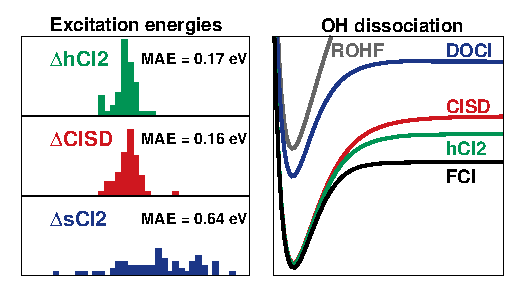
\includegraphics[keepaspectratio,width=2in]{TOC}}
%\end{center}
%\bigskip
\end{abstract}

% Title
\maketitle


%%%%%%%%%%%%%%%%%%%%%%%%%%%%%%%%%%%%%%%%%%%%%%%%%%
\section{Introduction}
\label{sec:intro}
%%%%%%%%%%%%%%%%%%%%%%%%%%%%%%%%%%%%%%%%%%%%%%%%%%


Configuration interaction (CI) offers a systematic way to solve the many-body electronic structure problem. \cite{SzaboBook,Helgakerbook}
By including progressively more determinants in the Hilbert space, the wave function becomes increasingly closer to the exact one, and so does the electronic energy.
In full CI (FCI), all determinants are accounted for and the problem is solved exactly (for a given basis set).
In practice, however, one resorts to approximate CI models, where only the determinants that satisfy a given criterion are included in the truncated Hilbert space.

The most well-known CI route is excitation-based.
Starting from a reference determinant, typically the Hartree-Fock (HF) determinant,
one generates all determinants that are connected to it by excitating at most $e$ electrons.
The excitation degree $e$ thus defines the order of the approximate CI model:
CI with single excitations (CIS); CI with single and double excitations (CISD), CI with single, double and triple excitations (CISDT), and so on.
A different CI route is based on the seniority number $s$ (the number of unpaired electrons in a given determinant).
In seniority-based CI (sCI) \cite{Bytautas_2011,Allen_1962,Smith_1965,Veillard_1967}, there is no reference determinant, and one accounts for all determinants having seniority equal or less than $s$.
For systems with an even number of electrons, the first approximate model is defined by $s=0$ (sCI0), usually refered to as doubly-occupied CI (DOCI),
which is followed by the higher-order models sCI2, sCI4, and so on.
For an odd number of electrons, the seniority route follows along odd numbers of $s$: sCI1, sCI3, and so on.
%Limited studies for radicals and excited states

%sCI works well to describe molecular dissociation \cite{Bytautas_2015,Alcoba_2014,Alcoba_2014b}
%For small systems, FCI is still attainable and one can thus gauge the performance of approximate CI models.
We have recently introduced a third CI route, hierarchy CI (hCI), \cite{Kossoski_2022}
where the Hilbert space is partitioned according to a hierarchy parameter $h$ that combines the excitation degree $e$ and the seniority number $s$ according to $h = (e+s/2)/2$.
For different properties and closed-shell molecular systems, 
hCI was found to display an overall faster convergence to the FCI results than the traditional excitation-based CI, as a function of the number of determinants $\Ndet$. \cite{Kossoski_2022}
However, hCI has only been defined for a closed-shell reference, thus systems with an even number of electrons.
Here, our first goal is to generalize hCI for open-shell systems and to assess the performance of this class of methods by performing calculations for various properties of several radicals.
%A generalization of the method for open-shell systems has not yet been proposed.
%excitations of increasingly higher order give rise to a systematically improvable sequence of CI methods:
The second goal is to evaluate how perturbation theory, more precisely the second-order Epstein-Nesbet (EN2) perturbative correction, \cite{Garniron_2019}
impacts different properties of ground-state closed-shell systems and radicals, for excitation-based, sCI and hCI methods.

%Whereas the first CI root represents the electronic ground state, higher-lying roots give access to excited states.
%Similarly, the favourable results of hCI when compared to excitation-based CI for ground states raises the question on how well it can describe excitation energies.
%The performance of excitation-based CI for excited states is well stablished, \cite{} but remains an open question for sCI methods,
Inspired by the results of hCI for ground-state closed-shell systems, \cite{Kossoski_2022} our third goal is to define and assess the accuracy of hCI models for excited states.
Finally, to the best of our knowledge, sCI models have not yet been directly used to target excited states,
despite the growing number of methods that exploit the concept of seniority number,
for both ground
\cite{Limacher_2013,Limacher_2014,Tecmer_2014,Boguslawski_2014a,Boguslawski_2015,Boguslawski_2014b,Boguslawski_2014c,Johnson_2020,Henderson_2014,Stein_2014,Henderson_2015,Chen_2015,Bytautas_2018,Marie_2021,Boguslawski_2021,Tecmer_2022,Mamache_2023} 
and excited states.
\cite{Boguslawski_2016b,Boguslawski_2016c,Boguslawski_2019,Nowak_2019,Kossoski_2021,Marie_2021,Tecmer_2022,Rishi_2023,Nowak_2023} 
Our fourth goal is therefore to introduce and gauge sCI models for excited states.
There are two possible approaches to target excited states with CI.
One can employ the ground-state HF orbitals and obtain excitation energies from the higher-lying eigenvalues of the CI matrix, which we refer to as ground-state based approach.
Instead, one may optimize the orbitals for the excited state of interest (described with an appropriate reference), followed by a separate CI calculation,
in a so-called state-specific approach ($\Delta$CI).
There has been a recent surge in the development of state-specific methods, covering 
single-reference and multiconfigurational self-consistent field,
\cite{Ziegler_1977,Burton_2021,Shea_2018,Tran_2019,Tran_2020,Hardikar_2020,Burton_2022,Hanscam_2022,Kossoski_2023,Marie_2023}
% add references for SCF
%\cite{Ziegler_1977,Burton_2021}
%multiconfigurational SCF, \cite{Shea_2018,Tran_2019,Tran_2020,Hardikar_2020,Burton_2022,Kossoski_2023,Marie_2023}
density functional theory, 
\cite{Filatov_1999,Kowalczyk_2011,Kowalczyk_2013,Gilbert_2008,Barca_2018,Hait_2020,Hait_2021,Hardikar_2020,Zhao_2020,Levi_2020,Carter-Fenk_2020,Toffoli_2022,Schmerwitz_2022}
and coupled-cluster 
\cite{Piecuch_2000,Mayhall_2010,Lee_2019,Kossoski_2021,Marie_2021,Rishi_2023}
methods.
In particular, by employing a minimal configuration state function reference, 
we have recently shown that excitation-based $\Delta$CI models deliver far more accurate excitation energies than the ground-state based analogues. \cite{Kossoski_2023}
Based on this promising set of results for excitation-based CI, here we explore both ground-state based and state-specific approaches for sCI and hCI models.




%%%%%%%%%%%%%%%%%%%%%%%%%%%%%%%%%
\section{Hierarchy configuration interaction}
\label{sec:hCI}
%%%%%%%%%%%%%%%%%%%%%%%%%%%%%%%%

%For an arbitrary reference Slater determinant, with seniority $s_0$, the hierarchy $h$ associated to a another determinant
With respect to a given reference Slater determinant, the hierarchy $h$ of a target determinant is defined as
\begin{equation}
        \label{eq:h}
        %h = \frac{e+\Delta s/2}{2},
	h = \frac{e+ (s-s_0)/2}{2},
\end{equation}
where $s$ and $s_0$ denote the seniority of target and reference determinants, respectively, and $e$ represents the excitation degree that connect the two determinants.
This definition renders a degree of dissimilarity between two determinants (reference and target),
which accounts for differences in orbital occupation (through the excitation degree $e$)
and differences in the number of unpaired electrons (through the term $(s-s_0)/2$).
The latter always assumes an integer value (for both even and odd numbers of electrons), such that $h$ becomes an integer or half-integer.
Also, Eq.~\eqref{eq:h} simplifies to the previous definition \cite{Kossoski_2022} for the case of a closed-shell reference determinant, when $s_0 = 0$.

state-specific methods
$\Delta$sCI2 
$\Delta$hCI1
From here on, labels carrying the $\Delta$ symbol denote a state-specific approach,
whereas those without imply the ground-state based approach.


%%%%%%%%%%%%%%%%%%%%%%%%%%%%%%%%%
\section{Computational details}
\label{sec:compdet}
%%%%%%%%%%%%%%%%%%%%%%%%%%%%%%%%

The hCI models introduced here were implemented in {\QP} \cite{Garniron_2019} through a straightforward modification of the
\textit{configuration interaction using a perturbative selection made iteratively} (CIPSI) algorithm. \cite{Huron_1973,Giner_2013,Giner_2015,Garniron_2018}
By allowing only for the determinants that are connected with the reference determinant(s) up to a given maximum hierarchy $h$,
the CIPSI algorithm is restricted to the truncated Hilbert space defined by the reference determinant(s) and the value of $h$.
{\QP} \cite{Garniron_2019} was also employed to perform all the CI calculations presented here.
In a given calculation, the energies are considered to be converged when the (largest) renormalized EN2 correction computed in the truncated Hilbert space 
lies below \SI{0.01}{\milli\hartree}. \cite{Garniron_2018}
%by spanning the most important regions of the truncated Hilbert space
This selected CI procedure requires considerably fewer determinants than the total number of determinants in the truncated Hilbert space,
while delievering fairly converged absolute and excitation energies.
The ground- and excited-state CI energies are obtained with the Davidson iterative algorithm. \cite{Davidson_1975}
For a given approximate CI model, we futher evaluated the bare and the renormalized EN2 perturbative correction. \cite{Garniron_2019} 
%associated with the determinants left outside the truncated space.
This calculation involves a single loop over the determinants left outside the truncated space but connected to it via at most double excitations.
Looping over these external doubly excited determinants thus represents an additional $\order*{N^4}$ factor on top of the computational scaling of the CI calculation.
For example, hCI2 and CISD present a $\order*{N^6}$ computational scaling, whereas hCI2+EN2 and CISD+EN2 scale as $\order*{N^{10}}$,
though with a small prefactor stemming from the EN2 calculation.

To gauge the performance of hCI against excitation-based and seniority-based CI for radical systems,
we have calculated the ground-state potential energy curves (PECs) for the dissociation of four radical systems:
\ce{OH}, \ce{CN}, vinyl (\ce{C2H3}), and \ce{H7}.
These calculations employed the ground-state restricted open-shell HF orbitals and the frozen core approximation.
%which display a variable number of bond breaking.
The equilibrium geometry of vinyl was taken from Ref.~\onlinecite{Loos_2020},
%also reproduced in the \SupInf,
and the PECs were computed along the \ce{C=C} double bond breaking coordinate, with the remaining internal coordinates kept frozen.
For \ce{H7}, we considered equally spaced and linearly arranged hydrogen atoms, and the PECs were computed along the symmetric dissociation coordinate.
The results were analyzed along the same lines of our report on hCI for closed-shell systems. \cite{Kossoski_2022}
Namely, for the different CI models considered here, 
we evaluated the convergence of the non-parallelity error (NPE), the distance error, the vibrational frequencies, and the equilibrium geometries, as functions of $\Ndet$.
The NPE (distance error) of a given level of theory is defined as the maximum minus (plus) the minimum differences between its corresponding PEC and the FCI one, for a given range of coordinates.
Details about how the vibrational frequencies and equilibrium geometries were obtained from the calculated PECs,
and the ranges defining the NPE and distance errors can be found in the \SupInf.

The various CI models introduced here were further assessed based on calculated vertical excitation energies for 60 electronic states,
from 18 closed-shell systems and 8 radicals, with geometries extracted from the QUEST database. \cite{Veril_2021}
The full set of excited states and calculated excitation energies, for the various CI models, are provided in the {\SupInf}.
We employed the aug-cc-pVDZ basis set for systems having up to three non-hydrogen atoms and the 6-31+G(d) basis set for the larger ones.
Core orbitals were frozen.
We performed calculations following both the standard ground-state based CI route and the state-specific CI route. \cite{Kossoski_2023}
For the latter, we employed the state-specific orbitals obtained in Ref.~\onlinecite{Kossoski_2023}.
In contrast to excitation-based CI, energies obtained with sCI and hCI models are not invariant under rotations withing the occupied and virtual subspaces.
The computed excitation energies were compared against the reference values provided in the QUEST database. \cite{Veril_2021}
%For completeness, we also reproduce the geometries in the \SupInf.



%%%%%%%%%%%%%%%%%%%%%%%%%%%%%%%%
\section{Results and discussion}
\label{sec:res}
%%%%%%%%%%%%%%%%%%%%%%%%%%%%%%%%


%%%%%%%%%%%%%%%%%%%%%%%%%%%%%%%%
\subsection{hCI for radicals}
\label{sec:res_A}
%%%%%%%%%%%%%%%%%%%%%%%%%%%%%%%%

% redefine the distance errors because of negative values?
% vinyl missing point at 5.2 for s3i+pt2 and at 2.0 for s5+pt2
% CN correct dissociating part for h4 and h3.5
% H8 missing points for Q+pt2
% H8 missing 9.0 for T+pt2

The full set of PECs for the open-shell systems (\ce{OH}, \ce{CN}, \ce{H7}, and vinyl) are presented in the {\SupInf},
along with the NPEs, distance errors, equilibrium geometries and vibrational frequencies, plotted as a function of $\Ndet$ for the different CI models.
The present results for open-shell systems are discussed in detail in the following,
and display similar trends to the ones previously reported for closed-shell systems. \cite{Kossoski_2022}
hCI typically improves the convergence of the different properties when compared to excitation-based CI.
Concerning the NPEs, such improvement is clear for \ce{OH} and \ce{CN} (involving a single bond breaking), less so for vinyl (double bond breaking),
whereas for \ce{H7} (multiple bond breaking), hCI and excitation-based CI perform similarly.
This behavior had also been observed for dissociation of closed-shell systems. \cite{Kossoski_2022}
The same trend is observed for the distance error, although the improvement from excitation-based CI to hCI is less marked than for the NPEs.
hCI further leads to a faster convergence of the equilibrium geometry of \ce{CN}, while comparable results are found for the geometries of the other systems.
Meanwhile, a clear improvement from excitation-based CI to hCI is observed for the vibrational frequencies, except for \ce{H7}, where no difference is found.

%orbital optimization?

We further assesssed the effect of the EN2 perturbative correction for both the open-shell systems studied here 
and the closed-shell systems (\ce{HF}, \ce{F2}, \ce{N2}, ethylene, \ce{H4}, and \ce{H8}) addressed in our first report on hCI. \cite{Kossoski_2022}
The full set of PECSs is shown in the {\SupInf}.
At stretched geometries, the perturbative correction can lead to kinks and large jumps in the PECs.
Such problems were encountered at some levels of CI for \ce{CN}, vinyl, \ce{H8}, and \ce{H7}, and to a less extent, for \ce{N2} (only for hCI1).
For the remaining five systems (\ce{HF}, \ce{F2}, ethylene, \ce{H4}, and \ce{OH}),
the EN2 correction produced smooth PECs at dissociation.
Around the equilibrium geometry, the perturbative correction produced well-behaved PECs at all levels of CI and for all systems, 
except for \ce{CN}, which is related to crossing of states around equilibrium.

We found that the EN2 perturbative correction generally reduces the errors of all observables considered here, for a given level of excitation-based CI and hCI routes.
As such, it accelerates the rate of convergence as a function of the excitation degree or hierarchy parameter.
Importantly, the perturbative corrected hCI route still outperforms the excitation-based counterpart, just as for the uncorrected comparison.
Furthermore, the reduction of the errors is overall more monotonic than without the perturbative correction,
which is illustrated in Fig.\ref{} for the particular case of \ce{F2}.
For the sCI route, however, the EN2 correction does not bring a clear improvement to render it competitive in relation to the excitation-based and hCI alternatives.

% rPT2 vs PT2 there are important differences

%xe
%\ce{OH} massive improvement
%\ce{CN} \ce{H4} \ce{N2} \ce{F2} \ce{HF} big improvement
%\ce{H7} \ce{H8} vinyl ethylene some improvement
 
%freq
%\ce{OH} massive improvement
%\ce{CN} \ce{F2} \ce{N2} \ce{H4} \ce{H7} big improvement
%\ce{HF} \ce{H8} vinyl ethylene some improvement


%%%%%%%%%%%%%%%%%%%%%%%%%%%%%%%%
\subsection{hCI for excited states}
\label{sec:res_B}
%%%%%%%%%%%%%%%%%%%%%%%%%%%%%%%%

In Tab.~\ref{tab:1} we present the statistical errors of the different methods, organized by their computational scaling.
% hCI1 and hCI1.5
We found that $\Delta$hCI2 and $\Delta$CISD display comparable MAEs, despite the somewhat more favourable MSE and RMSE of the latter.
This means that the additional determinants present in the former model recover a larger fraction of the correlation energy for excited state than for the ground state,
thus creating a bias toward underestimated excitation energies.
Even though this unbalance is still observed for $\Delta$hCI2, it is much less serious than observed for the lower-order state-specific hCI methods.


\begin{table}[ht!]
\caption{Mean Signed Error (MSE), Mean Absolute Error (MAE), and Root-Mean Square Error (RMSE) in Units of eV, with Respect to Reference Theoretical Values, for the Set of 
38 Singly Excited States of Closed-Shell Systems and 
Listed in the {\SupInf}.
}
\label{tab:1}
\begin{ruledtabular}
\begin{tabular}{lddd}
method            & \mc{1}{c}{MSE} & \mc{1}{c}{MAE} & \mc{1}{c}{RMSE} \\
\hline
$\Delta$CSF       & -0.75 & 0.81 & 0.95 \\
CIS               & +0.03 & 0.62 & 0.63 \\
\hline
hCI1              & +1.08 & 1.12 & 1.25 \\
$\Delta$hCI1      & -1.37 & 1.41 & 1.52 \\
hCI1.5            & +1.95 & 1.95 & 2.03 \\
$\Delta$hCI1.5    & -2.95 & 2.95 & 3.14 \\
$\Delta$CISD      & -0.13 & 0.17 & 0.22 \\
$\Delta$hCI2      & -0.19 & 0.20 & 0.25 \\
\hline
sCI2/sCI2         & +1.40 & 1.40 & 1.53 \\
sCI2/sCI0         & -0.22 & 0.42 & 0.57 \\
$\Delta$sCI2/sCI2 & +0.74 & 0.77 & 0.85 \\
$\Delta$sCI2/sCI0 & -0.88 & 0.88 & 0.96 \\
\end{tabular}
\end{ruledtabular}
\end{table}

\begin{table}[ht!]
\caption{Mean Signed Error (MSE), Mean Absolute Error (MAE), and Root-Mean Square Error (RMSE) in Units of eV, with Respect to Reference Theoretical Values, for the Set of 
16 Singly-Excited States from Open-Shell Doublets 
Listed in the {\SupInf}.
}
\label{tab:2}
\begin{ruledtabular}
\begin{tabular}{lddd}
method            & \mc{1}{c}{MSE} & \mc{1}{c}{MAE} & \mc{1}{c}{RMSE} \\
\hline
$\Delta$CSF       & -0.09 & 0.50 & 0.67 \\
CIS               & +0.30 & 0.41 & 0.55 \\
\hline
hCI1              & +0.76 & 0.80 & 1.02 \\
$\Delta$hCI1      & -0.09 & 0.58 & 0.94 \\
hCI1.5            & +1.22 & 1.22 & 1.45 \\
$\Delta$hCI1.5    & -0.26 & 0.66 & 0.92 \\
$\Delta$CISD      & +0.00 & 0.16 & 0.23 \\
$\Delta$hCI2      & -0.03 & 0.14 & 0.19 \\
\hline
sCI1              & +0.27 & 0.44 & 0.66 \\
$\Delta$sCI1      & -0.15 & 0.28 & 0.40 \\
\end{tabular}
\end{ruledtabular}
\end{table}

Despite the rather poor performance of lower-order hCI models for excitation energies,
we further investigated whether higher-order versions could be competitive against the traditional excitation-based counterparts.
For that, we performed calculations for a subset of 14 excited states of small molecular systems (\ce{H2O}, \ce{BF}, \ce{HCF}, \ce{HCl}, and \ce{N2}),
with corresponding statistical errors shown in Tab.~\ref{tab:2}.
Even though this is a small set, it should be enough to obtain the main trends on the accuracy of higher-order models.


\begin{table}[ht!]
\caption{Mean Signed Error (MSE), Mean Absolute Error (MAE), and Root-Mean Square Error (RMSE) in Units of eV, with Respect to Reference Theoretical Values,
for the Set of 14 Singly Excited States of Closed-Shell Systems Listed in the {\SupInf}.
}
\label{tab:2}
\begin{ruledtabular}
\begin{tabular}{lddd}
method            &     \mc{1}{c}{MSE} & \mc{1}{c}{MAE} & \mc{1}{c}{RMSE} \\
\hline
CISD              & +4.09 & 4.09 & 4.18  \\
CISDT             & +0.09 & 0.18 & 0.20  \\
CISDTQ            & +0.14 & 0.14 & 0.16  \\
%
$\Delta$CISD      & -0.13 & 0.17 & 0.21  \\
$\Delta$CISDT     & -0.19 & 0.19 & 0.23  \\
$\Delta$CISDTQ    & -0.02 & 0.02 & 0.02  \\
%
hCI2              & +2.89 & 3.00 & 3.28  \\
hCI2.5            & +1.93 & 1.93 & 2.05  \\
hCI3              & +0.18 & 0.18 & 0.19  \\
%
$\Delta$hCI2      & -0.22 & 0.22 & 0.27  \\
$\Delta$hCI2.5    & -0.27 & 0.27 & 0.30  \\
$\Delta$hCI3      & -0.21 & 0.21 & 0.24  \\
$\Delta$hCI3.5    & -0.08 & 0.08 & 0.09  \\
\end{tabular}
\end{ruledtabular}
\end{table}

%We found that the errors of both ground-state based hCI and state-specific $\Delta$hCI to systematically decrease when going toward higher orders of $h$, which would be expected.
%Unfortunately, the pace of decrease is too slow to render these approaches very useful.
%In line with what has been found for excitation-based CI \cite{Kossoski_2023}, 

The case of $\Delta$hCI2 was discussed above for the larger set of excitation energies.
Here we further notice that hCI2 was found to be somewhat more accurate than CISD, even though the errors are still too large.
However, this improvement does not reflect on the state specific route (compare $\Delta$hCI2 and $\Delta$CISD in Tabs.~\ref{tab:1} and ~\ref{tab:2}).
Moving to the next order, even though the state-specific route ($\Delta$hCI2.5) is far more accurate than the ground-state based route (hCI2.5),
it is actually less accurate then $\Delta$hCI2.
An improved performance is found for hCI3, $\Delta$hCI3, CISDT, and $\Delta$CISDT, which present quite similar MAEs and RMSEs.
There is thus no advantage in moving from excitation-based to hCI at this order, similarly to what discussed before for the $\Delta$hCI2 and $\Delta$CISD models.
Moreover, $\Delta$hCI3 is not more accurate than hCI3, as also observed for $\Delta$CISDT and CISDT. \cite{Kossoski_2023}
We notice, however, that the state-specific models present negative MSEs, in contrast to the positives values obtained in the ground-state based route.
This reflects an umbalanced description of correlation effects, favoring the excited states.
At the next order, $\Delta$hCI3.5 has significantly smaller errors, but at a much more elevated computational cost.


%%%%%%%%%%%%%%%%%%%%%%%%%%%%%%%%
\subsection{Seniority CI for excited states}
\label{sec:res_C}
%%%%%%%%%%%%%%%%%%%%%%%%%%%%%%%%

We refer to Tab.~\ref{tab:1} and ~\ref{tab:2} to discuss the performance of seniority-based CI for excited states.
sCI2 delivers quite poor results (MAE of \SI{1.06}{eV}), whereas $\Delta$sCI2 reduces the statistical errors (MAE of \SI{0.60}{eV}).
This improvement, however, is not as expressive as observed for excitataion-based and hierarchy-based methods.
Compare, for instance, with the cases of hCI2.5 and $\Delta$hCI2.5 shown in Tab.~\ref{tab:1}.
The large errors, even following the state-specific approach, combined with the formal $\order*{e^N}$ scaling of these methods,
render seniority-based CI unsuitable for calculations of excitation energies.

pCCD-CI for excited states \cite{Nowak_2023}

%%%%%%%%%%%%%%%%%%%%%%%%%%%%%%%%
\section{Conclusion}
\label{sec:ccl}
%%%%%%%%%%%%%%%%%%%%%%%%%%%%%%%%

%three CI routes (excitation, hierarchy, and seniority-based).
%Here we address the knowledge gaps outlined above by setting four goals.
%Extending our previous findings for closed-shell \cite{Kossoski_2022} to open-shell systems,
%We further explored Epstein-Nesbet second-order perturbative corrections to the various approximate CI methods.
%The second is to assess the performance of this method for ground state radicals, similarly to what has been done for closed-shell systems. \cite{Kossoski_2022}

%The third goal is to assess the improvement from perturbative corrections to ground-state radicals and closed-shell systems, for both excitation-based and hierarchy-based CI methods.
%For hCI and excitation-based CI, the perturbative correction tends to accelerate and stabilize the convergence of different properties toward the FCI results.
%EN2 perturbative corrections lead to faster and more monotonic convergence of different properties
%We have considered both closed and open shell systems, considering ground-state properties and excitation energies, for a diverse set of molecular systems.
%Finally, we introduce and gauge seniority-based and hierarchy-based CI methods for excited states, along both the standard ground-state based route and the state-specific route. \cite{Kossoski_2023}

Here we have generalized hCI \cite{Kossoski_2022} for the case of an open-shell reference determinant, thus extending its applicability to radical species and excited states.
By surveying the dissociation of several open-shell systems, 
we found that the hCI route has an edge in comparison to excitation-based CI, for both weakly correlated (equilibrium geometries) and strongly correlating (dissociation) regimes.
Meanwhile, seniority-based CI leads to far less accurate results in comparison to hCI or excitation-based CI, for a given computational cost.
These findings are in line with what had been found for closed-shell systems. \cite{Kossoski_2022}
We also found that, for closed- and open-shell systems,
the EN2 perturbative corrections lead to substantial improvements for hCI and excitation-based CI routes (while keeping the upper hand for the former), but do not help much with the deficiencies of the sCI route.

We further gauged the performance of hCI and sCI methods, based on either HF ground-state orbitals or state-specific orbitals, to describe excited states of closed-shell systems and radicals.
Despite their elevated computational cost, sCI models produced relatively poor results (even in a state-specific approach), and thus should not be useful in practice.
Similarly, for lower orders of hCI (hCI1 and hCI1.5), the performance is very poor,
with ground-state (state-specific) orbitals leading to largely overestimated (underestimated) excitation energies.
The situation improves at the state-specific $\Delta$hCI2 order, even though its accuracy is somewhat worse than $\Delta$CISD, both models sharing the same computational scaling. 
Unfortunately, $\Delta$hCI2.5 does not lead to more accurate results, whereas all the CI models at next next order (CISDT, $\Delta$CISDT, hCI3, and $\Delta$hCI3) show comparable performance.
Overall, hCI models for excited states are either innacurate given their computational cost ($h=1$, $h=1.5$ and $h=2.5$) or comparable to excitation-based CI at the same order ($h=2$ and $h=3$).
%it is fair to conclude that 



%%%%%%%%%%%%%%%%%%%%%%%%%%%%%%%%
\begin{acknowledgements}
This work was performed using HPC resources from CALMIP (Toulouse) under allocation 2021-18005.
This project has received funding from the European Research Council (ERC) under the European Union's Horizon 2020 research and innovation programme (Grant agreement No.~863481).
\end{acknowledgements}
%%%%%%%%%%%%%%%%%%%%%%%%%%%%%%%%

%%%%%%%%%%%%%%%%%%%%%%%%%%%%%%%%%%
\section*{Supporting information available}
\label{sec:SI}
%%%%%%%%%%%%%%%%%%%%%%%%%%%%%%%%%%

%%%%%%%%%%%%%%%%%%%%%%%%%%%%%%%%
%\section*{Data availability statement}
%%%%%%%%%%%%%%%%%%%%%%%%%%%%%%%%
%The data that support the findings of this study are openly available in Zenodo at \href{http://doi.org/XX.XXXX/zenodo.XXXXXXX}{http://doi.org/XX.XXXX/zenodo.XXXXXXX}.

%%%%%%%%%%%%%%%%%%%%%%%%%%%%%%%%
\bibliography{manuscript}
%%%%%%%%%%%%%%%%%%%%%%%%%%%%%%%%

\end{document}
